\documentclass[border=2pt]{standalone}
\usepackage{tikz}
\usetikzlibrary{automata,arrows.meta}

\begin{document}
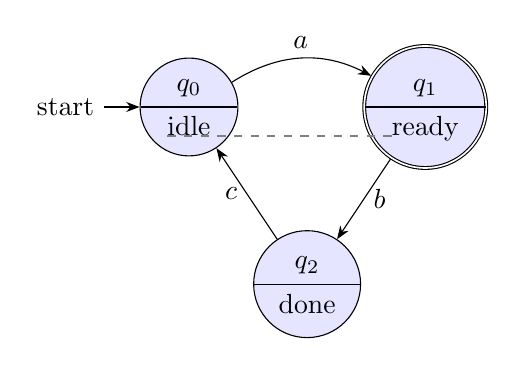
\begin{tikzpicture}[>=Stealth,every state/.style={fill=blue!10}]
  \node[state with output,initial] (idle) at (0,0) {$q_0$\nodepart{lower}idle};
  \node[state with output,accepting] (ready) at (3,0) {$q_1$\nodepart{lower}ready};
  \node[state with output] (done) at (1.5,-2.25) {$q_2$\nodepart{lower}done};
  \path[->] (idle) edge[bend left] node[above] {$a$} (ready)
             (ready) edge node[right] {$b$} (done)
             (done) edge node[left] {$c$} (idle);
  \draw[gray,dashed] (idle.lower) -- (ready.lower);
\end{tikzpicture}
\end{document}
